% ===== 原文 pp.33--41（PDF p.43--51）：第 4 章 拓扑场论、范畴与 2-范畴 =====
% ===== 本文件 ch04-01.tex：印刷 pp.33--36（PDF p.43--46） =====
% 本章无编号公式；全部显示公式用 \[ … \]，一律不编号。

% [原文 p.33]
\chapter{拓扑场论、范畴与 2-范畴}

到目前为止，我们讨论了一些具体的上同调 4d TFT 的例子。它们的可观测量谱被证明带有丰富的代数结构，而不同 TFT 之间的对偶关系则蕴含这些代数结构之间的非平凡等价。本章我们通过回顾\emph{所有} 4d TFT 共有的特征，为分析这些结构作准备。

% [Tutor Note: p.33 “余维 $k$ 的缺陷带 $(n-k)$-范畴结构”这条规律可用来自检全章断言：$n=4$ 时余维 1（边界条件）给 3-范畴、余维 2（面算子）给 2-范畴、余维 3（线算子）给 1-范畴即普通范畴；§4.3 说 3d TFT 的边界条件构成 2-范畴、§4.4 说 4d 面算子构成 2-范畴，都符合 $n-k$。]

事实上，当人们把一个 4d TFT 放在具有非平凡边界 $\partial M$ 的流形 $M$ 上时，必须沿 $\partial M$ 对场施加边界条件。所有这类边界条件的集合被证明带有一种非常丰富的代数结构，称为\emph{3-范畴}（3-category），下面我们就来解释。人们也可以考虑更高余维的缺陷；例如余维二的\emph{面算子}。它们同样带有一种代数结构，称为\emph{2-范畴}；研究这个 2-范畴的一个自然办法，是把 4d TFT 在圆周上紧化为一个有效的 3d TFT。类似地，可以把 4d TFT 在 2-球面上紧化到二维，来研究余维三的\emph{线算子}。

因此，为了理清一个 4d TFT 中编码的信息，人们自然被引向研究低维的 TFT。本章我们系统地回顾二维、三维与四维 TFT 所附带的范畴结构。

\section{二维 TFT 与膜范畴}

对我们来说，范畴是代数的一种推广，即“具有许多对象的代数”。也就是说，代替一个带有乘法映射 $V\otimes V\to V$ 的向量空间 $V$，我们有一个集合 $\Ob$、一族向量空间 $V_{\mathsf{A}\mathsf{B}}$（$\mathsf{A},\mathsf{B}\in\Ob$），以及复合映射 $V_{\mathsf{A}\mathsf{B}}\otimes V_{\mathsf{B}\mathsf{C}}\to V_{\mathsf{A}\mathsf{C}}$。这些复合映射必须在显然的意义下是结合的。特别地，对每个 $\mathsf{A}$，空间 $V_{\mathsf{A}\mathsf{A}}$ 是一个（可能非交换的）代数。我们另外假定所有这些代数都带有单位元。

集合 $\Ob$ 称为对象集，向量空间 $V_{\mathsf{A}\mathsf{B}}$ 称为态射空间。

% [原文 p.34]
$V_{\mathsf{A}\mathsf{A}}$ 的元素称为 $\mathsf{A}$ 的自同态，$V_{\mathsf{A}\mathsf{A}}$ 称为 $\mathsf{A}$ 的自同态代数。通常记 $V_{\mathsf{A}\mathsf{B}}=\Mor(\mathsf{A},\mathsf{B})$ 与 $V_{\mathsf{A}\mathsf{A}}=\Mor(\mathsf{A},\mathsf{A})=\End(\mathsf{A})$。在物理应用中，这些向量空间总是复的，而且通常具有整分次（由某种 $U(1)$ 荷给出）。

% [Tutor Note: p.34 的“整分次”不是范畴公理的一部分，而是物理上的额外数据：B-模型中它来自向量丛复形的同调度，A-模型中来自 Maslov 指标（见第 7 章 §7.6）。自洽检验：图 4.1--4.2 的复合必须满足 $\deg(\cO_{\mathsf{A}\mathsf{B}}\cdot\cO_{\mathsf{B}\mathsf{C}})=\deg\cO_{\mathsf{A}\mathsf{B}}+\deg\cO_{\mathsf{B}\mathsf{C}}$，因为 $\Mor$ 的复合是分次映射。]

至今已众所周知，2d TFT 中边界条件的集合具有范畴的结构。这个范畴的对象集 $\Ob$ 就是边界条件的集合，而向量空间 $V_{\mathsf{A}\mathsf{B}}$ 是该 TFT 在带边界条件 $\mathsf{A}$ 与 $\mathsf{B}$ 的（定向）区间上的状态空间。态射的复合来自两件事实：其一，空间 $V_{\mathsf{A}\mathsf{B}}$ 可以解释为坐在边界两段交接处的局部算子所构成的空间，这两段分别带边界条件 $\mathsf{A}$ 与 $\mathsf{B}$（图 4.1）；其二，局部算子之间可以彼此融合（图 4.2）。

\begin{figure}[htbp]
\centering
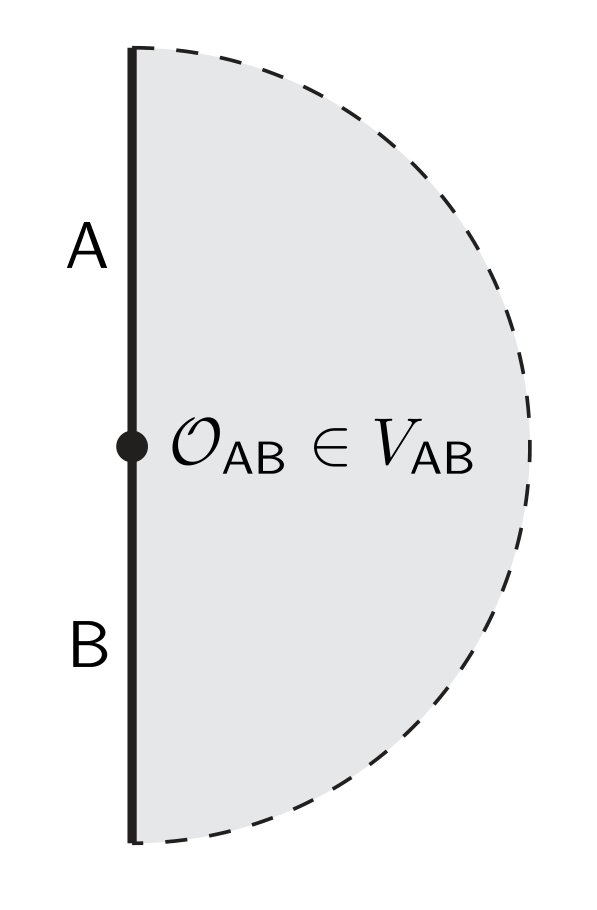
\includegraphics[width=0.38\textwidth]{fig41.png}
\figtitle{4.1}{边界条件范畴中的态射对应于位于两段边界交接处的局部算子。}
\end{figure}

\begin{figure}[htbp]
\centering
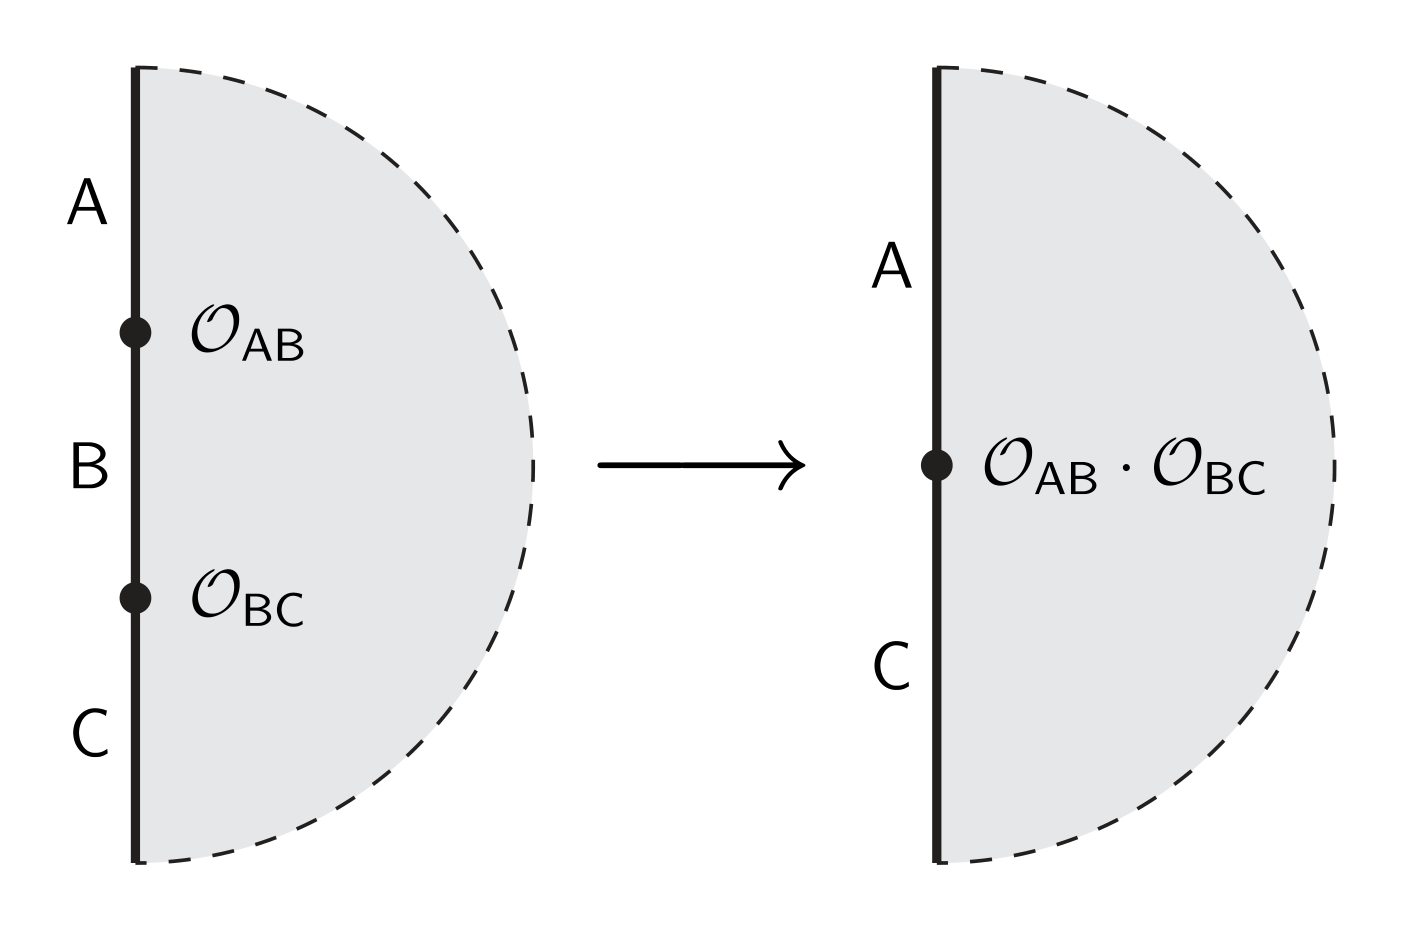
\includegraphics[width=0.48\textwidth]{fig42.png}
\figtitle{4.2}{态射的复合通过把局部算子的插入点合并来实现。我们用 $\cdot$ 表示这一运算。}
\end{figure}

在数学文献中，通常用带标记的点表示对象，用连接这些点的箭头表示向量空间 $V_{\mathsf{A}\mathsf{B}}$ 的元素。从物理观点看，更自然的做法是用一条定向直线上带标记的线段表示对象，用坐在相邻两段交接处的点表示态射。

% [原文 p.35]
让我们回想两个对我们重要的、简单的 2d TFT 例子。第一个是靶空间为 $X$ 的 B-模型，其中 $X$ 是带有全纯体积形式的复流形（即一个可能非紧的 Calabi-Yau 流形）。相应的边界条件范畴被论证为等价于 $X$ 上凝聚层的有界导出范畴，记作 $D^b(\operatorname{Coh}(X))$。它的对象可以看成 $X$ 上全纯向量丛的复形，或 $X$ 的复子流形。第二个是靶空间为 $Y$ 的 A-模型，其中 $Y$ 是辛流形。相应的边界条件范畴被认为等价于 Fukaya-Floer 范畴的某个版本。它最简单的对象是 $Y$ 的拉格朗日子流形，其上配备带平坦联络的酉向量丛。在二维的语境中，人们通常把边界条件称为膜（brane），并谈论 A-膜与 B-膜。

% [Tutor Note: p.35 强调 $X$ 带有\emph{全纯}体积形式的用处：它蕴含 $c_1(X)=0$，即 Calabi-Yau 条件，这是 B-模型无反常（$c_1=0$ 使单圈反常相消）从而能作为 2d TFT 良好定义的前提（作者用 “has been argued”，因为 B-模型 ↔ $D^b(\operatorname{Coh} X)$ 是 Kontsevich 同调镜像对称猜想的一侧，A-模型 ↔ Fukaya 范畴一侧仍属猜想）。自洽检验：取 $X$ 为一点，$D^b(\operatorname{Coh}(\mathrm{pt}))$ 就是有限维分次向量空间范畴，与“平凡 2d TFT 的膜范畴”相符。]

A-模型与 B-模型即使在二维也没有穷尽所有可能性。在第 7 章我们会遇到其他不那么熟悉的 2d TFT 及其膜范畴。

\section{二维 TFT 与 2-范畴}

2d TFT 的边界可以视为一个非平凡 TFT 与一个平凡 TFT 之间的边界。更一般地，可以考虑任意一对 2d TFT 之间的边界。这样的边界可以称为缺陷线（defect line），或壁（wall）。固定一对 TFT 之间所有壁的集合具有范畴的结构。为看出这一点，记 $\mathbb{X}$ 与 $\mathbb{Y}$ 为我们选定的那对 TFT，并用 $\bar{\mathbb{X}}$ 表示把 $\mathbb{X}$ 的宇称反转后得到的理论。把世界面沿壁所在的位置折回去（见图 4.3），我们看到：$\mathbb{X}$ 与 $\mathbb{Y}$ 之间的壁，等同于理论 $\bar{\mathbb{X}}\times\mathbb{Y}$ 的一个边界。于是我们可以援用前面的讨论，断定壁是范畴 $\mathbb{V}_{\mathbb{X}\mathbb{Y}}$ 的对象。

\begin{figure}[htbp]
\centering
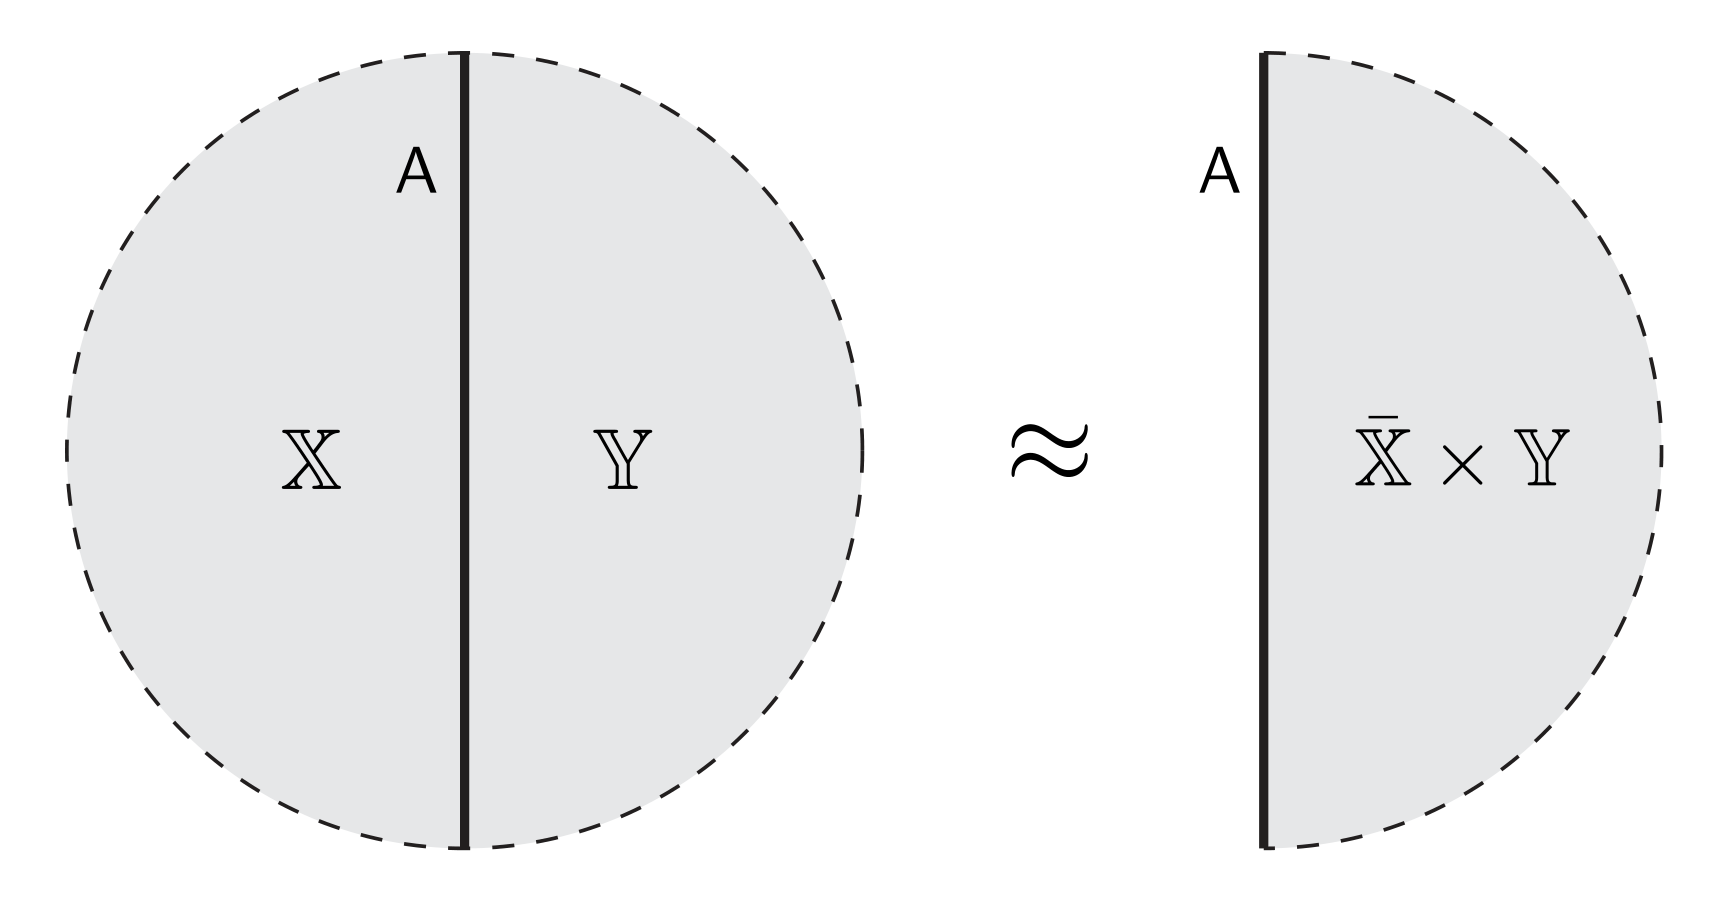
\includegraphics[width=0.7\textwidth]{fig43.png}
\figtitle{4.3}{分隔理论 $\mathbb{X}$ 与 $\mathbb{Y}$ 的壁，等价于理论 $\bar{\mathbb{X}}\times\mathbb{Y}$ 的一个边界。}
\end{figure}

% [Tutor Note: p.35 的“折叠”论证补全如下：壁是 $\Sigma$ 中把世界面分成两块的一条线段 $\ell$；沿 $\ell$ 折叠使 $\mathbb{X}$ 那一块被 $\bar{\mathbb{X}}$ 覆盖——宇称反转恰好抵消折叠造成的定向翻转，于是折叠后的世界面只剩一块、以 $\ell$ 为边界，其内部的理论是 $\bar{\mathbb{X}}\times\mathbb{Y}$。自洽检验：取 $\mathbb{X}=\mathbb{Y}$，则 $\bar{\mathbb{X}}\times\mathbb{X}$ 的边界条件给出 $\mathbb{X}$ 的缺陷线，与本节末“缺陷线构成单对象 2-范畴”一致。]

任给两个壁 $\mathsf{A},\mathsf{B}\in\Ob(\mathbb{V}_{\mathbb{X}\mathbb{Y}})$，从 $\mathsf{A}$ 到 $\mathsf{B}$ 的态射空间就是可以插在 $\mathsf{A}$ 与 $\mathsf{B}$ 交接处的局部算子所构成的空间。态射的复合则通过融合坐在缺陷线上的局部算子得到。

% [原文 p.36]
壁的集合上有一个显然的“融合”运算：给定理论 $\mathbb{X}$ 与 $\mathbb{Y}$ 之间的一个壁，以及理论 $\mathbb{Y}$ 与 $\mathbb{Z}$ 之间的一个壁，我们可以把它们融合起来，得到理论 $\mathbb{X}$ 与 $\mathbb{Z}$ 之间的一个壁（图 4.4）。用数学语言描述这一情形，就是说 2d TFT 的集合具有 2-范畴的结构。一个 2-范畴有对象、态射与 2-态射（态射之间的态射）。在目前的情形，对象是 2d TFT；从对象 $\mathbb{X}$ 到对象 $\mathbb{Y}$ 的态射集合是理论 $\mathbb{X}$ 与 $\mathbb{Y}$ 之间壁的集合。壁的融合给出复合态射的一种方式。给定同一对 TFT 之间的任意两个壁，它们之间的 2-态射空间就是可以插在这两个壁交接处的局部算子所构成的空间。

\begin{figure}[htbp]
\centering
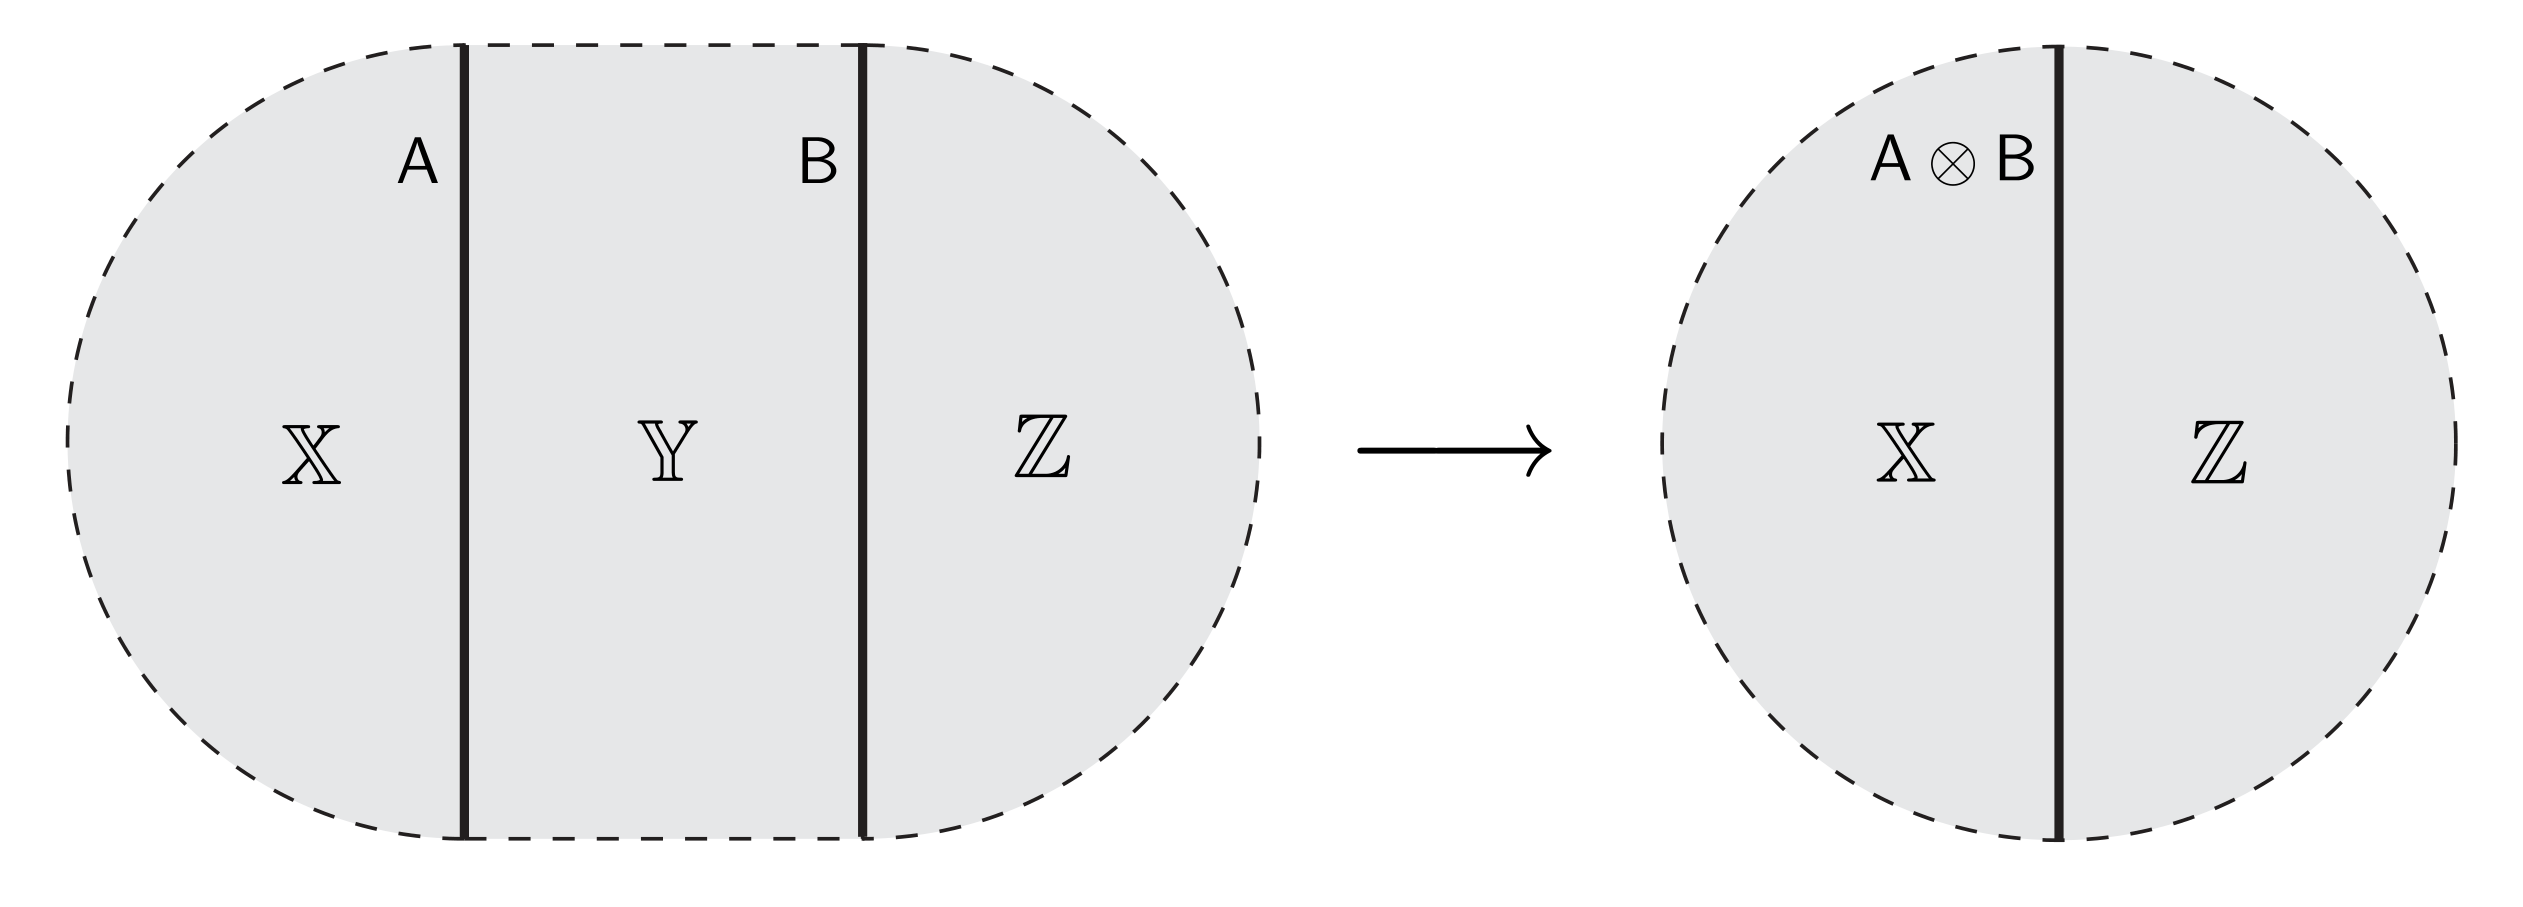
\includegraphics[width=0.85\textwidth]{fig44.png}
\figtitle{4.4}{2d TFT 的 2-范畴的 1-态射对应于壁，1-态射的复合对应于融合壁。这一运算记作 $\otimes$。}
\end{figure}

也可以换一种稍有不同的说法：一个 2-范畴有一族对象（在我们的情形即 2d TFT），并且对任意一对对象 $\mathbb{X}$、$\mathbb{Y}$ 有一个态射范畴 $\mathbb{V}_{\mathbb{X}\mathbb{Y}}$（在我们的情形即壁的范畴）。壁的融合意味着存在“复合”态射范畴的方式。也就是说，给定范畴 $\mathbb{V}_{\mathbb{X}\mathbb{Y}}$ 的一个对象 $\mathsf{A}$ 与范畴 $\mathbb{V}_{\mathbb{Y}\mathbb{Z}}$ 的一个对象 $\mathsf{B}$，有一条规则确定范畴 $\mathbb{V}_{\mathbb{X}\mathbb{Z}}$ 的一个对象 $\mathsf{A}\otimes\mathsf{B}$。这还不是全部；人们不仅能融合壁，还能融合壁上插入了局部算子的壁（图 4.4）。这就确定了 2-态射上的复合映射。这个新的复合不同于把局部算子看作范畴 $\mathbb{V}_{\mathbb{X}\mathbb{Y}}$ 中态射时的复合。这些复合映射具有若干性质，盯着融合壁的图、并用度规无关性即可推出。例如，新旧两种复合相互交换，如图 4.5 所示。

% [Tutor Note: p.36 “（图 4.4）”疑为笔误，此处讲的是把局部算子插在壁上再融合，对应的应是图 4.5（图 4.4 画的是 1-态射即壁本身的融合）。另外，“新旧两种复合相互交换”正是 2-范畴（双范畴）的交换律（interchange law）；图 4.6 中由四个角沿两条不同路径到达同一结果，就是这条交换律的几何证明。]

即使只关心某一个特定的 TFT，2-范畴的概念也是有用的。具体地说，一个 2d TFT 中的缺陷线构成一个只有一个对象的 2-范畴。此时只有一个态射范畴 $\mathbb{V}_{\mathbb{X}\mathbb{X}}$，而它带有额外的结构，其来源是：融合两条缺陷线给出同一理论中的另一条缺陷线。这一结构使人可以定义如下的“张量”规则：
